{
{\sffamily Det er meget svært at kvantificere, hvorvidt det gyldne snit
bliver brugt i malerkunsten, men vi kan opstille nogle hypoteser for,
hvilke resultater vi ville forvente, hvis det gyldne snit bliver brugt.
De følgende hypoteser antager derfor den generelle opfattelse, at det
gyldne snit er specielt æstetisk tiltalende.
}

\begin{hypotese}
    Mere end $50\%$ af de analyserede malerier, har én eller flere
    regioner liggende i det gyldne snit.
    \label{hypo_binaer}
\end{hypotese}

\begin{hypotese}
    Antallet af regioner i de fire snit tilknyttet snitratioen
    $\varPhi$, afviger ikke mere end $\pm10\%$ fra hinanden.
    \label{hypo_fire_g_snit}
\end{hypotese}

\begin{hypotese}
    Vi må have, at mere end en tredjedel malerierne har et lærred, hvis
    dimensioner er lig $\varphi\pm2.4\%$.
    \label{hypo_golden_ractangle}
\end{hypotese}

\begin{hypotese}
    Antallet af detekterede regioner i det gyldne snit, er skarpt
    større, end antallet i alle andre snit.
    \label{hypo_alle_andre_snit}
\end{hypotese}

\begin{hypotese}
    Antallet regioner liggende i det gyldne snit, er skarpt større, end
    antallet af regioner liggende i snittet ved to tredjedele.
    \label{hypo_to_tredjedele}
\end{hypotese}

\begin{hypotese}
    Antallet regioner liggende i det gyldne snit, er skarpt større, end
    antallet af regioner liggende det midterste snit.
    \label{hypo_midten}
\end{hypotese}

\begin{hypotese}
    Vi må have, at antallet af regioner liggende i det gyldne snit,
    tidsperioder imellem, højest kan afvige med $\pm10\%$.
	\label{hypo_tid}
\end{hypotese}

\begin{hypotese}
    Antallet af regioner liggende i det gyldne snit, nationaliteter
    imellem, højest kan afvige med $\pm10\%$.
	\label{hypo_nation}
\end{hypotese}

\begin{hypotese}
    Antallet af regioner liggende i det gyldne snit, afviger ikke fra
    antallet af regioner i snittet ved to tredjedele, med mere end
    $15\%$.
	\label{hypo_15p}
\end{hypotese}

Ovenstående samling af hypoteser kan give os et billede af, hvorvidt det
gyldne snit kunne være brugt, når vi analyserer et datasæt. Vi vil
derfor kaste et blik på hvilke malerier vi har til rådighed i vores
kørsel.

\subsection{Datasæt}
Det korpus, vi kører vores analyse på, består af billeder hentet fra
``The Web Gallery of Art''\cite{wgahu}, som er en online billededatabase, med
europæiske kunstartikler fra år 1001 -- 1900. I kunstartiklerne, hvor
det samlede antal er omkring 23.000, indgår møbler, kalkmalerier,
skulpturer, mosaikker og malerier, hvor sidstnævnte, vil være vores
fokus. Over halvdelen af disse kunstartikler står udstillet på museum.
Databasen blev oprettet i 1996, med det formål at præsentere kunst fra
renæssancen (ca.  14. -- 17.  århundrede), men blev senere udvidet, til
også at inkludere kunst fra andre perioder. Dette betyder, at
størstedelen af malerierne vi undersøger, er fra tidsperioden 1450 --
1650 og er malet af italienske kunstnere. Endvidere er langt de fleste
malerier, klassificeret som religiøse.  Disse informationer er givet fra
WGA, men er også suppleret i bilag \ref{appendix_grafer} som
grafer.

Vi må af ovenstående grunde forvente, at resultater, fra en analyse på
vores datasæt, vil være farvet af samlingen af malerier, og det derfor
kan være svært at drage nogen konklusioner for malerkunsten generelt, da
resultaterne vil være begrænset, til kun at gælde for et udsnit af
vestlig kultur. Endvidere findes der ingen nyere malerier i datasættet,
hvilket gør at vi ikke kan udtale os om nyere malerkunst.

Billederne, som suppleres fra databasen, er af høj kvalitet, men der er
visse problemer, som vi nævner nedenfor.

\begin{itemize}
    \item \textbf{Beskæring af billeder}\\
        Vi kan ikke vide os sikre på, om billederne i datasættet er
        ordentligt beskåret, hvilket betyder at vi \emph{kan} have, at
        noget af billedrammen er med i billedet. Dette kan muligvis
        volde lidt problemer med udtrækning af regioner, men hvad værre
        er, så gør det vores mål, for hvor det gyldne snit ligger,
        upræcist. Dette har vi dog taget højde for, i kraft af vores
        margin.  Endeligt er der inkluderet billeder af malerier
        detaljer i databasen, som er udsnit af maleriet, således at
        målene på billedet ikke passer.
    \item \textbf{Forvrængning og perspektiv}\\
        Billederne af malerier er taget med et kamera, hvor linsen muligvis kan
        forvrænge billedet. Vi kan derfor have skæve linjer og tage
        forkerte beslutninger, for regioner, pga. dette. Endvidere kan
        billedet være taget skævt, således at billedet hælder til den
        ene side. Vi kan selvfølgelig også have at perspektivet i
        billedet er forkert, fordi billedet er taget fra en skæv vinkel.
    \item \textbf{Opdelte malerier}\\
        Nogle store malerier kan være blevet opdelt, da databasen har
        det formål at vise malerierne på en computerskærm, hvor meget
        store billeder kan være svære at betragte. Dette betyder, at
        nogle billeder ikke viser hele maleriet, men blot er et udsnit,
        hvilket påvirker vores muligheder for at sige noget fornuftigt
        om det gyldne snit i maleriet.
\end{itemize}

Nogle stilarter, såsom kalkmalerier og tegninger, har gennem
udokumenterede afprøvninger, vist sig at være besværlige at analysere,
pga. meget svingende farvegengivelse. Endvidere, kan disse være billeder
af en hvælving i en kirke, som ikke egner sig til analyse for det gyldne
snit. Vi har derfor valgt kun at analysere malerier, kendetegnet ved at
de er beskrevet som ``painting'' fra WGA.

Alt det ovenstående vil påvirke resultaterne, ved analyse på vores
datasæt.

\subsection{Eksperimentsopstilling}
I \ref{chap_afproevning} er de optimale tærskelværdier fundet.  Idet
denne hypotese blot kigger på frekvensen for brug af det gyldnesnit mod
andre snit, hvis eneste restriktion er at de skal have et fælles forhold
til det gyldnesnit.  Det er også fordelagtigt at maksimere antallet af
andre snit, da det giver et bedre grundlag for eksperimentet.  Afstanden
mellem to snit er begrænset af margin defineret til at være
$2.4\%$, som beskrevet i kapitlet \ref{margin}.  Denne margin skal være tilstede på begge sider af
et snit, så derfor vil hvert snit fylde $(2.4*2)\%$.  Det maksimale
antal af snit på et billede må altså være $100/4.8=20.833$.
Med en margin på $2.4\%$ vil der være en strimmel på $0.1\%$ af
billedet, som ikke bliver brugt.Og mellem to marginer vil der derfor ligge en
strimmel på $0.2\%$. 

Den eneste undtagelse findes ved midten, i udregningen
\ref{label_midt_udregning} ses først hvordan snittet til venstre for
midten findes, og derefter hvor lang afstanden er mellem de to snit.
\begin{equation}\label{resul_midt_udregningen}
    1-0.518 = 0.482
    0.518-0.482 = 0.036
\end{equation}
Der er altså en stimmel på $0.048-0.036 = 0.012 = 1.2\%$ af
billedet, hvor interessante regioner potentielt kunne blive talt to gange.
Dette er illustreret i billede \ref{resultat_fejl_midt}.
\begin{figure}[!h]
	\centering
	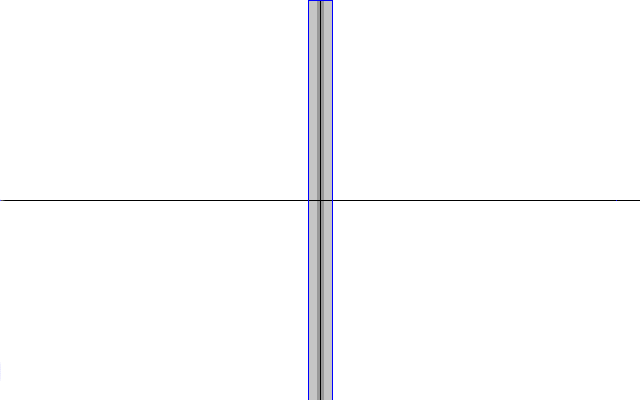
\includegraphics[scale=0.5]{afsnit/resultater/billeder/midt_strimmel}
	\label{resultat_fejl_midt}
\end{figure}

}
% vim: set tw=72 spell spelllang=da:
